In this chapter, we analyze two proposed idealized models of the TCPC. These models are designed to incorporate key geometric modifications identified as beneficial in reducing energy dissipation, as described in \cite{Rijnberg2018}. These modifications, summarized in Figure~\ref{fig:positive_modifications}, serve as a foundation for investigating the effects of caval offsetting, curving, flaring, and other geometric factors on flow dynamics.

\begin{figure}[H]
	\centering
	\vspace{3mm}
	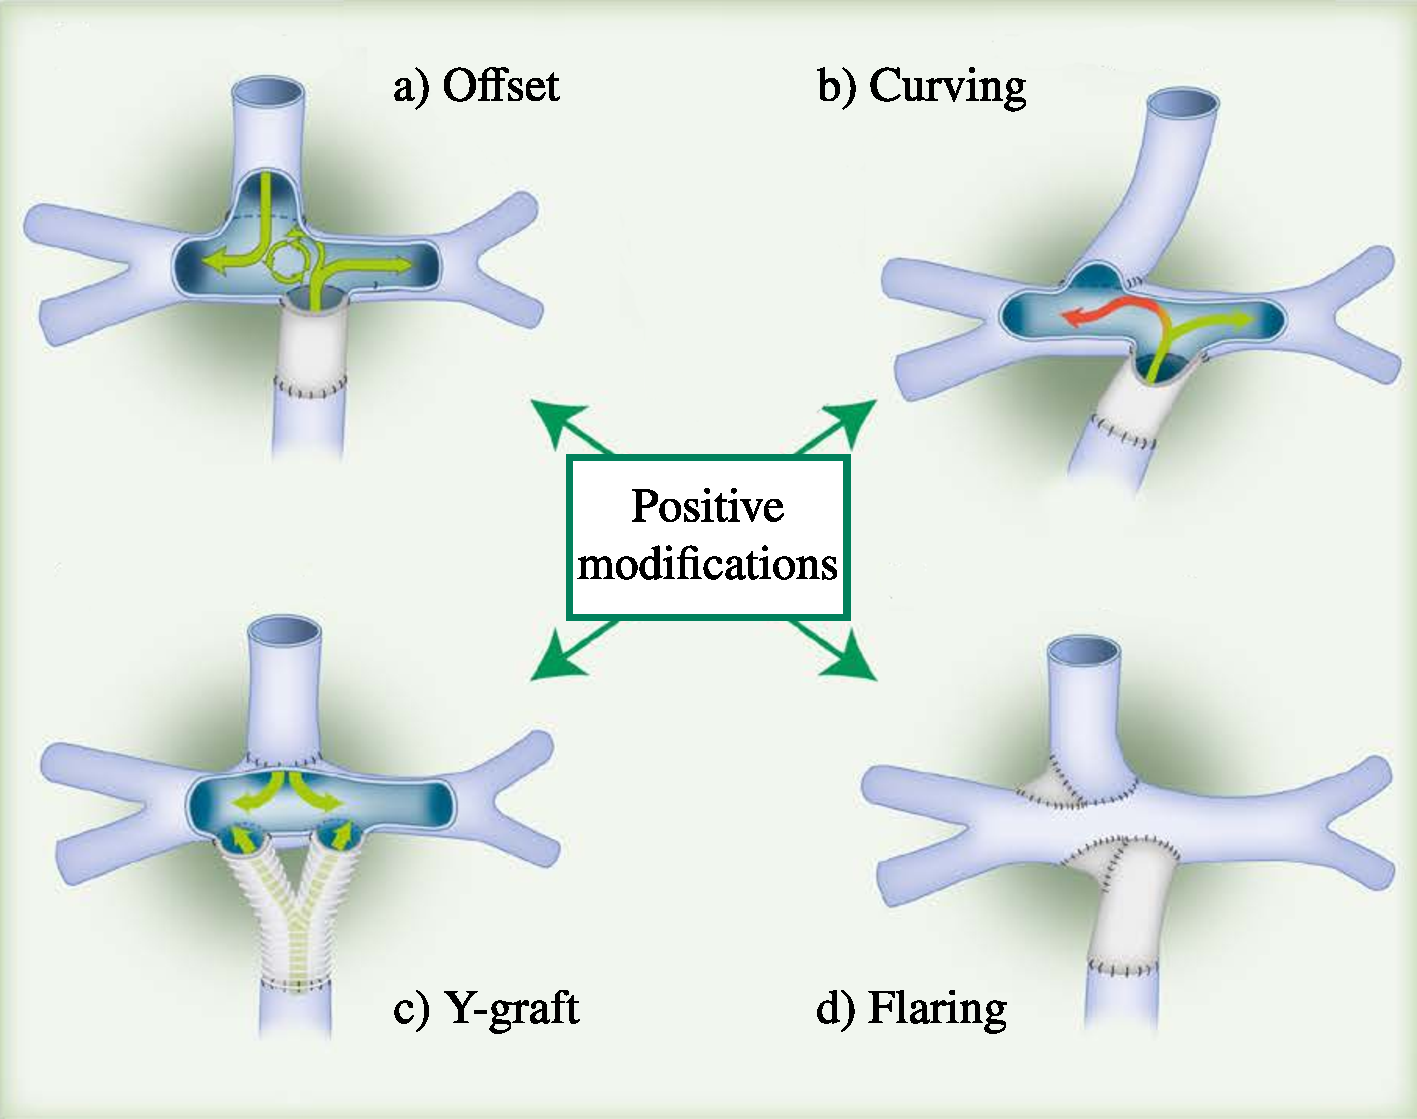
\includegraphics[width=0.65\textwidth]{figures/energyloss-en.pdf}
	\vspace{3mm}
	\caption[Positive Modifications for TCPC]{Key modifications to improve TCPC geometry and reduce energy dissipation: a) caval offsetting, where the inferior and superior vena cava are misaligned to minimize flow collision; b) curving, where the vessels are curved; c) the Y-graft configuration, which splits the flow evenly between outlets; and d) flaring, where the connections are widened to reduce sharp corners and flow resistance. Adapted from \cite{Rijnberg2018}.}
	\label{fig:positive_modifications}
\end{figure}


